\paperchapter{October 2014}{October 2014}{A}{60}{GSET 2014}
\keytable{\kcell{1}{C} & \kcell{2}{A} & \kcell{3}{C} & \kcell{4}{B} & \kcell{5}{B} & \kcell{6}{D} & \kcell{7}{D} & \kcell{8}{A} & \kcell{9}{C} & \kcell{10}{A} \\
\kcell{11}{D} & \kcell{12}{A} & \kcell{13}{D} & \kcell{14}{C} & \kcell{15}{B} & \kcell{16}{B} & \kcell{17}{D} & \kcell{18}{B} & \kcell{19}{C} & \kcell{20}{C} \\
\kcell{21}{C} & \kcell{22}{B} & \kcell{23}{C} & \kcell{24}{D} & \kcell{25}{B} & \kcell{26}{A} & \kcell{27}{B} & \kcell{28}{A} & \kcell{29}{D} & \kcell{30}{D} \\
\kcell{31}{C} & \kcell{32}{B} & \kcell{33}{C} & \kcell{34}{B} & \kcell{35}{A} & \kcell{36}{C} & \kcell{37}{A} & \kcell{38}{A} & \kcell{39}{B} & \kcell{40}{D} \\
\kcell{41}{A} & \kcell{42}{C} & \kcell{43}{A} & \kcell{44}{D} & \kcell{45}{A} & \kcell{46}{B} & \kcell{47}{D} & \kcell{48}{C} & \kcell{49}{A} & \kcell{50}{D} \\
\kcell{51}{C} & \kcell{52}{A} & \kcell{53}{B} & \kcell{54}{C} & \kcell{55}{A} & \kcell{56}{A} & \kcell{57}{C} & \kcell{58}{D} & \kcell{59}{A} & \kcell{60}{D}}
\begin{question}{1}
{Which of the following is least desirable outcome of teaching in higher education?\par}
\optsone{Enhancement of independent thinking of students}{Increase in students probing skills}{Good preparation for appearing in examination}{Helping students to think out of the box}
\answer{C}{Good preparation for appearing in examination}
\begin{explain}
Higher education aims at independent thinking, inquiry (probing), creativity and ``thinking out of the box''. Mere \textbf{preparation for examinations} is the \emph{least desirable} outcome: it encourages rote learning.
\end{explain}
\end{question}

\begin{question}{2}
{Here some qualities of the teachers are presented. Which one of the following combination of qualities is most suitable in an effective teacher?\newline (1) Knowledge of subject matter\newline (2) Effective oral communication\newline (3) Pleasant presence\newline (4) To be object of respect of the students\newline (5) To be object of respect of the leaders of the society\par}
\optsfour{1, 2, 4}{1, 2, 3}{2, 3, 4}{1, 2, 5}
\answer{A}{1, 2, 4}
\begin{explain}
An effective teacher combines \textbf{mastery of the subject (1)}, \textbf{effective oral communication (2)} and \textbf{the respect of students (4)}. Being respected by society's leaders (5) and a pleasant presence (3) are not essential qualities of teaching. The answer is 1, 2, 4.
\end{explain}
\end{question}

\begin{question}{3}
{Which of the following technique of teaching is more suitable for developing creativity in students?\par}
\optstwo{Lecture}{Demonstration}{Field study}{Providing self-learning material}
\answer{C}{Field study}
\begin{explain}
\textbf{Field study} puts learners in real, open-ended situations where they observe, explore, question and produce original ideas, which develops creativity.
\why{Lecture and demonstration are teacher-centred; self-learning material is structured and convergent.}
\end{explain}
\end{question}

\begin{question}{4}
{Assessment that take place during process of teaching in classroom is:\par}
\optstwo{Classroom assessment}{Formative assessment}{Summative assessment}{Comprehensive assessment}
\answer{B}{Formative assessment}
\begin{explain}
\textbf{Formative assessment} takes place \emph{during} the teaching--learning process to monitor progress and provide feedback (assessment \emph{for} learning). Summative assessment comes at the end.
\end{explain}
\end{question}

\begin{question}{5}
{Which of the following helps learner to learn better?\par}
\optstwo{Giving notes}{Discussion in the class}{Explaining the main points}{Knowledge of the teacher}
\answer{B}{Discussion in the class}
\begin{explain}
\textbf{Classroom discussion} involves learners actively: they express, question, listen and build on others' ideas. This deepens understanding far more than passively receiving notes or explanations.
\end{explain}
\end{question}

\begin{question}{6}
{In constructivist approach, learner is viewed as:\par}
\optstwo{responding being}{evolving being}{emotional being}{exploring being}
\answer{D}{exploring being}
\begin{explain}
In \textbf{constructivism} (Piaget, Vygotsky, Bruner) the learner is an active \textbf{explorer} who constructs knowledge through exploration and experience. The learner is not a passive responder.
\end{explain}
\end{question}

\begin{question}{7}
{When each unit of a population has an equal likelihood of being selected, the method of sampling is called:\par}
\optstwo{A non-random sampling}{A quota sampling}{A snowball sampling}{A random sampling}
\answer{D}{A random sampling}
\begin{explain}
When every unit of the population has an \textbf{equal (and independent) chance} of selection, the method is \textbf{random (probability) sampling}.
\end{explain}
\end{question}

\begin{question}{8}
{A researcher wants to study the future of an Institution. For the study which tool is most appropriate for him/her?\par}
\optsfour{Questionnaire}{Observation}{Interview}{Rating Scale}
\answer{A}{Questionnaire}
\begin{explain}
Studying the future of an institution requires the considered views of many stakeholders and experts. A \textbf{questionnaire} can collect these systematically from a large, spread-out group; futures studies such as the \emph{Delphi technique} use successive rounds of questionnaires to build consensus about the future.
\end{explain}
\end{question}

\begin{question}{9}
{Hypothesis cannot be stated in:\par}
\optstwo{Null and question form}{Declarative terms}{General terms}{Directional form}
\answer{C}{General terms}
\begin{explain}
A research hypothesis is a specific, testable statement. It can be declarative, null or directional, but it \textbf{cannot be in question form}. (A question is a research \emph{question}, not a hypothesis.)
\end{explain}
\end{question}

\begin{question}{10}
{A text taken from a source is placed in a research report without providing reference is called as:\par}
\optstwo{Plagiarism}{Popularism}{Perfectionism}{Post-referencism}
\answer{A}{Plagiarism}
\begin{explain}
Presenting someone else's text without acknowledging the source is \textbf{plagiarism}.
\end{explain}
\end{question}

\begin{question}{11}
{What is the correct sequence of steps in research?\par}
\optsone{Sampling; identification of problem; development of tools; data analysis; data collection}{Identification of problem; development of tools; sampling; data collection; data analysis}{Development of tools; identification of problem; data analysis; sampling; data collection}{Identification of problem; sampling; development of tools; data collection; data analysis}
\answer{D}{Identification of problem; sampling; development of tools; data collection; data analysis}
\begin{explain}
The logical research sequence: \textbf{identify the problem $\rightarrow$ select the sample $\rightarrow$ develop tools $\rightarrow$ collect data $\rightarrow$ analyse data}, which is option (D).
\tip{Some texts place tool development before sampling. Either way, the problem comes first and data analysis comes after data collection.}
\end{explain}
\end{question}

\begin{question}{12}
{Practitioners such as teachers, counsellors and other professionals attempt to find solutions to some issues in a systematic manner. This is known as:\par}
\optstwo{Action Research}{Basic Research}{Applied Research}{Developmental Research}
\answer{A}{Action Research}
\begin{explain}
\textbf{Action research} (Stephen Corey applied it to education) is carried out by practitioners such as teachers and counsellors to solve \emph{their own immediate problems} systematically and improve practice.
\end{explain}
\end{question}

\begin{context}
\textbf{Read the paragraph and answer the Question Nos.~13--18.}\par\smallskip
Adolescence is a period of rapid growth and development bridging childhood and adulthood. Practicing healthy eating behaviour is one of the most important factors to meet the nutritional needs of adolescents. Proper eating behaviours that are learned in early life are maintained in adulthood thus reducing the risk of major chronic diseases. Physical and psychological changes occurring during this period usually significantly influence their dietary behaviours. As teens become more independent, they make more of their own food choices. However, being influenced by a massive amount of factors (biological, social, physical, economic, psychological beliefs and knowledge about food) and changing of lifestyle may affect their dietary choices and eating behaviour, thus making them fail to adhere to healthy eating practices. Peer pressure in colleges leads adolescents to eating non-nutritional foods like pizzas and burgers. Due to irregular college schedules, intake of caffeinated drinks increases and water intake reduces. Poor nutrition can lead to reduced concentration in studies, low stamina, depression or poor posture.
\end{context}
\begin{question}{13}
{Adolescents succumb to unhealthy dietary habits due to:\par}
\optstwo{Physical and psychological changes}{Independence in making food choices}{Changing lifestyle}{Peer pressure in colleges}
\answer{D}{Peer pressure in colleges}
\begin{explain}
The official key gives \textbf{peer pressure in colleges}: ``Peer pressure in colleges \textbf{leads} adolescents to eating non-nutritional foods like pizzas and burgers.'' This is the direct cause the passage names for giving in to unhealthy foods.
\end{explain}
\end{question}

\begin{question}{14}
{Unhealthy dietary habits means:\par}
\optstwo{Eating pizzas and burgers}{Caffeinated drinks}{Poor nutritional diet}{Drinking less water}
\answer{C}{Poor nutritional diet}
\begin{explain}
Pizzas, burgers, caffeine and less water are examples. What they add up to is a \textbf{poor nutritional diet}, the general meaning of unhealthy dietary habits.
\end{explain}
\end{question}

\begin{question}{15}
{Reduced concentration in studies is because of:\par}
\optsone{Nature of Adolescent period}{Not being able to meet nutritional needs}{Influence of factors like biological and psychological}{Eating of foods like pizzas and burgers}
\answer{B}{Not being able to meet nutritional needs}
\begin{explain}
``\textbf{Poor nutrition} can lead to reduced concentration in studies.'' Poor nutrition means \textbf{not being able to meet nutritional needs}.
\end{explain}
\end{question}

\begin{question}{16}
{The author marks adolescent as bridging childhood and adulthood because it is a:\par}
\optsone{Period of independence in making dietary choices}{Period of physical and psychological changes}{Period of changing lifestyle}{Period of peer pressure}
\answer{B}{Period of physical and psychological changes}
\begin{explain}
Adolescence bridges childhood and adulthood because it is a period of rapid growth, i.e.\ \textbf{physical and psychological changes}.
\end{explain}
\end{question}

\begin{question}{17}
{What is the meaning of dietary behaviour?\par}
\optstwo{Taking different types of diet}{Taking caffeinated drinks}{Knowledge of different types of diets}{Making choices about diet}
\answer{D}{Making choices about diet}
\begin{explain}
Dietary behaviour refers to how a person \textbf{makes choices about diet}: what, when and how much to eat (``as teens become more independent, they make more of their own food choices'').
\end{explain}
\end{question}

\begin{question}{18}
{As per the author, how does dietary behaviour in adolescence affect health in adulthood?\par}
\optsone{Major chronic diseases are transferred from early stage to adulthood}{The seed of ill health in adulthood is sown by diet in early stages}{Dietary habits of adolescence are carried out in adulthood}{Dietary habits are maintained throughout life}
\answer{B}{The seed of ill health in adulthood is sown by diet in early stages}
\begin{explain}
``Proper eating behaviours that are learned in early life are maintained in adulthood, thus reducing the risk of major chronic diseases.'' By the same logic, poor eating in adolescence \textbf{sows the seeds of ill health in adulthood}.
\end{explain}
\end{question}

\begin{question}{19}
{Which one of the following functions a sender would perform during communication?\par}
\optsfour{Decoding}{Feedback}{Encoding}{Reception}
\answer{C}{Encoding}
\begin{explain}
The sender \textbf{encodes}: converts ideas into symbols (words, signs). Decoding and reception are the receiver's functions; feedback is the receiver's response.
\end{explain}
\end{question}

\begin{question}{20}
{Given the following components of communication, which combination represents classroom communication best?\newline (i) Individual to Individual\newline (ii) Individual to Group\newline (iii) Group to Individual\newline (iv) Group to Group\par}
\optstwo{(i) and (ii)}{(ii) and (iv)}{(i), (ii) and (iii)}{(iii) and (iv)}
\answer{C}{(i), (ii) and (iii)}
\begin{explain}
In a classroom the teacher speaks to individual students \textbf{(i)} and to the whole class \textbf{(ii)}, and the class or a group responds to the teacher \textbf{(iii)}. The answer is (i), (ii) and (iii).
\end{explain}
\end{question}

\begin{question}{21}
{In order to protect sensitive matter sent through e-mail, the sender should:\par}
\optstwo{write the matter in another language}{not provide self-address}{encrypt the matter}{not inform any one about this matter}
\answer{C}{encrypt the matter}
\begin{explain}
\textbf{Encryption} converts the content into a code that only the intended recipient (with the key) can read, protecting sensitive e-mail matter.
\end{explain}
\end{question}

\begin{question}{22}
{A manager of an organisation transfers a message to his/her subordinates. Which type of communication is this?\par}
\optsfour{Diagonal}{Downward}{Horizontal}{Upward}
\answer{B}{Downward}
\begin{explain}
Communication from a superior to subordinates is \textbf{downward communication}.
\end{explain}
\end{question}

\begin{question}{23}
{In what type of communication, sender transfers message using body movements?\par}
\optsfour{Verbal}{Written}{Gestural}{Silence}
\answer{C}{Gestural}
\begin{explain}
Communication through body movements (gestures, postures) is \textbf{gestural} (kinesic) non-verbal communication.
\end{explain}
\end{question}

\begin{question}{24}
{Arrange the elements of communication in a sequential order:\par}
\optstwo{Sender, receiver, message, feedback}{Sender, message, feedback, receiver}{Sender, feedback, message, receiver}{Sender, message, receiver, feedback}
\answer{D}{Sender, message, receiver, feedback}
\begin{explain}
\textbf{Sender $\rightarrow$ Message $\rightarrow$ Receiver $\rightarrow$ Feedback}.
\end{explain}
\end{question}

\begin{question}{25}
{If 2 $\times$ 7 = 41, 4 $\times$ 3 = 21, 5 $\times$ 5 = 52, then 3 $\times$ 6 = \blank{}\par}
\optsfour{39}{81}{121}{208}
\answer{B}{81}
\begin{explain}
The product is written with its digits reversed:
\[2\times7=14\rightarrow41,\qquad4\times3=12\rightarrow21,\qquad5\times5=25\rightarrow52\]
\[3\times6=18\rightarrow\mathbf{81}\]
\end{explain}
\end{question}

\begin{question}{26}
{Arrange in a meaningful sequence:\newline (1) Status\newline (2) Service\newline (3) Income\newline (4) Settlement\newline (5) Study\par}
\optsfour{5 $\rightarrow$ 2 $\rightarrow$ 3 $\rightarrow$ 1 $\rightarrow$ 4}{5 $\rightarrow$ 4 $\rightarrow$ 3 $\rightarrow$ 2 $\rightarrow$ 1}{4 $\rightarrow$ 3 $\rightarrow$ 2 $\rightarrow$ 1 $\rightarrow$ 5}{3 $\rightarrow$ 1 $\rightarrow$ 2 $\rightarrow$ 4 $\rightarrow$ 5}
\answer{A}{5 $\rightarrow$ 2 $\rightarrow$ 3 $\rightarrow$ 1 $\rightarrow$ 4}
\begin{explain}
A person first \textbf{studies (5)}, then gets \textbf{service} (a job) (2), which brings \textbf{income (3)}, which gives \textbf{status (1)}, and finally \textbf{settlement (4)} in life. The order is 5 $\rightarrow$ 2 $\rightarrow$ 3 $\rightarrow$ 1 $\rightarrow$ 4.
\end{explain}
\end{question}

\begin{question}{27}
{Put the correct number in the box:\newline 0, 2, 6, 12, [ ], 30\par}
\optsfour{18}{20}{28}{14}
\answer{B}{20}
\begin{explain}
Each term is $n(n-1)$: $1\cdot0=0$, $2\cdot1=2$, $3\cdot2=6$, $4\cdot3=12$, $5\cdot4=\mathbf{20}$, $6\cdot5=30$. (Differences: 2, 4, 6, 8, 10.)
\end{explain}
\end{question}

\begin{question}{28}
{If NOT is encoded as 415102, then SRP will have the code:\par}
\optsfour{918161}{191816}{1986}{689}
\answer{A}{918161}
\begin{explain}
Each letter is replaced by its alphabet position written \emph{in reverse}: N $=14\rightarrow41$, O $=15\rightarrow51$, T $=20\rightarrow02$, giving 415102.
SRP: S $=19\rightarrow91$, R $=18\rightarrow81$, P $=16\rightarrow61$, giving \textbf{918161}.
\end{explain}
\end{question}

\begin{question}{29}
{If 2 $\times$ 6 = 7, 4 $\times$ 2 = 27, 7 $\times$ 3 = 144, then 5 $\times$ 8 = \blank{}\par}
\optsfour{140}{142}{143}{144}
\answer{D}{144}
\keynote{No single consistent rule fits all three given examples. Students should record the official answer and not spend exam time on such items.}
\begin{explain}
The official key gives \textbf{(D) 144}. The first two examples fit $(b+1)^{a-1}$: $(6+1)^{2-1}=7$ and $(2+1)^{4-1}=27$. The third ($7\times3=144$) does not fit that rule, and no rule gives any of the options for $5\times8$ unambiguously. The question is best treated as defective; answer according to the key.
\end{explain}
\end{question}

\begin{question}{30}
{Complete the sequence by filling the blank using correct number:\newline 0, 2, 12, \blank{}, 80\par}
\optsfour{66}{52}{48}{36}
\answer{D}{36}
\begin{explain}
Each term is $n^2(n+1)$ for $n=0,1,2,3,4$: $0$, $1\cdot2=2$, $4\cdot3=12$, $9\cdot4=\mathbf{36}$, $16\cdot5=80$.
\end{explain}
\end{question}

\begin{question}{31}
{Put the correct number at "?" and complete the sequence:\newline A(4), F(9), M(?), Q(20)\par}
\optsfour{12}{14}{16}{17}
\answer{C}{16}
\begin{explain}
The number is the letter's position $+3$: A(1)$+3=4$, F(6)$+3=9$, M(13)$+3=\mathbf{16}$, Q(17)$+3=20$.
\end{explain}
\end{question}

\begin{question}{32}
{Complete the sequence by putting the correct letter:\newline C, H, M, \blank{}, W\par}
\optsfour{O}{R}{Q}{T}
\answer{B}{R}
\begin{explain}
The letters advance by 5: C(3), H(8), M(13), \textbf{R(18)}, W(23).
\end{explain}
\end{question}

\begin{context}
There are total 400 candidates applying for admission to one of the courses C1, C2, C3, C4 and C5, for study. The given table shows \% number of all 400 candidates admitted to these courses. Based on this table, answer the following questions (33--35):
\begin{center}
\begin{tabular}{lcccccc}\toprule \textbf{Course} & C1 & C2 & C3 & C4 & C5\\\midrule
\textbf{\% admitted} & 15 & 10 & 25 & 30 & 20\\
\textbf{Number} (of 400) & 60 & 40 & 100 & 120 & 80\\\bottomrule
\end{tabular}
\end{center}
\end{context}
\begin{question}{33}
{The sequence in increasing order of number of candidates in these courses, is:\par}
\optstwo{30, 65, 85, 90, 130}{35, 60, 80, 105, 120}{40, 60, 80, 100, 120}{50, 60, 70, 90, 130}
\answer{C}{40, 60, 80, 100, 120}
\begin{explain}
The numbers are 60, 40, 100, 120 and 80. In increasing order: \textbf{40, 60, 80, 100, 120}.
\end{explain}
\end{question}

\begin{question}{34}
{The ratio of number of candidates in course C3 to the number of candidates in course C5 is:\par}
\optsfour{3 : 2}{5 : 4}{6 : 4}{6 : 5}
\answer{B}{5 : 4}
\begin{explain}
C3 : C5 $=100:80=\mathbf{5:4}$ (equivalently $25\%:20\%$).
\end{explain}
\end{question}

\begin{question}{35}
{The sequence of admitted number of candidates, in order of courses C1 to C5, is:\par}
\optstwo{60, 40, 100, 120, 80}{50, 80, 100, 120, 50}{100, 50, 30, 130, 90}{90, 50, 30, 130, 100}
\answer{A}{60, 40, 100, 120, 80}
\begin{explain}
C1 to C5 in order: $15\%, 10\%, 25\%, 30\%, 20\%$ of 400 $=$ \textbf{60, 40, 100, 120, 80}.
\end{explain}
\end{question}

\begin{context}
The following graph records the number of employees who joined and left a company in the month of April, from the period 2005 to 2009. The initial number of employees in the company is 1000. Based on this graph, answer the questions 36--38.
\begin{center}
\begin{tikzpicture}
\begin{axis}[width=9cm,height=4.6cm,xmin=2004.5,xmax=2009.5,ymin=0,ymax=300,xtick={2005,...,2009},
  x tick label style={/pgf/number format/1000 sep=},tick label style={font=\scriptsize},
  ylabel={\scriptsize No.\ of employees},legend style={font=\tiny,at={(1.02,1)},anchor=north west}]
\addplot[mark=triangle*,thick,accent] coordinates {(2005,150) (2006,250) (2007,200) (2008,100) (2009,200)};
\addplot[mark=o,thick,brand] coordinates {(2005,200) (2006,150) (2007,100) (2008,150) (2009,100)};
\legend{Left,Joined}
\end{axis}
\end{tikzpicture}
\end{center}
\end{context}
\begin{question}{36}
{The ratio of total number of employees in 2005 to the total number of employees in 2006 is:\par}
\optsfour{11 : 10}{20 : 17}{21 : 19}{13 : 11}
\answer{C}{21 : 19}
\begin{explain}
Running total (start $=1000$):
\begin{center}\small
\begin{tabular}{lcccc}\toprule Year & Joined & Left & Net & Employees\\\midrule
2005 & 200 & 150 & $+50$ & \textbf{1050}\\ 2006 & 150 & 250 & $-100$ & \textbf{950}\\ 2007 & 100 & 200 & $-100$ & 850\\ 2008 & 150 & 100 & $+50$ & 900\\ 2009 & 100 & 200 & $-100$ & 800\\\bottomrule
\end{tabular}
\end{center}
2005 : 2006 $=1050:950=\mathbf{21:19}$.
\end{explain}
\end{question}

\begin{question}{37}
{How many employees were serving the company in 2005?\par}
\optsfour{1050}{1200}{1150}{900}
\answer{A}{1050}
\begin{explain}
$1000+200-150=\mathbf{1050}$ (see the table in Q.~36).
\end{explain}
\end{question}

\begin{question}{38}
{In which year, the number of employees was maximum?\par}
\optsfour{2005}{2007}{2008}{2009}
\answer{A}{2005}
\begin{explain}
The totals are 1050, 950, 850, 900 and 800, so the maximum is in \textbf{2005}.
\end{explain}
\end{question}

\begin{question}{39}
{Which of the following diagrams indicates all possible relations amongst milk-M, Sugar-S, Tea-T and Coffee-F?\par}
\optsfour{\tikz[baseline=-0.5ex,scale=0.32]{\draw (0,1.05) circle(1); \draw (-1.05,0) circle(1); \draw (1.05,0) circle(1); \draw (0,-1.05) circle(1);}}{\tikz[baseline=-0.5ex,scale=0.32]{\draw (0,0.8) circle(1); \draw (-0.8,0) circle(1); \draw (0.8,0) circle(1); \draw (0,-0.8) circle(1);}}{\tikz[baseline=-0.5ex,scale=0.32]{\draw (0,0) circle(2); \draw (0.3,0) circle(1.3); \draw (0.5,0.5) circle(0.4); \draw (0.5,-0.5) circle(0.4);}}{\tikz[baseline=-0.5ex,scale=0.32]{\draw (0,0) circle(2); \draw (0,-0.2) circle(1.4); \draw (-0.45,-0.5) circle(0.4); \draw (0.45,-0.5) circle(0.4);}}
\answer{B}{\tikz[baseline=-0.5ex,scale=0.32]{\draw (0,0.8) circle(1); \draw (-0.8,0) circle(1); \draw (0.8,0) circle(1); \draw (0,-0.8) circle(1);}}
\begin{explain}
Milk, sugar, tea and coffee are four different items that are commonly \emph{combined} in any mixture: milk with tea, sugar with coffee, tea with milk and sugar, and so on. To show \textbf{all possible} combinations, including one region common to all four, we need four \textbf{mutually overlapping circles} with a shared central region, as in diagram (B).
\end{explain}
\end{question}

\begin{question}{40}
{(i) Rohit possesses four two-wheelers\newline (ii) Two two-wheelers are black\newline (iii) One two-wheeler is a bicycle\newline From the above statements which conclusion can be drawn?\newline (I) Rohit has black bicycle\newline (II) Rohit has three scooters\newline (III) Rohit does not like black color.\par}
\optstwo{I and II}{III only}{II only}{None of I, II, III is true}
\answer{D}{None of I, II, III is true}
\begin{explain}
From ``two two-wheelers are black'' and ``one is a bicycle'' we cannot tell whether the bicycle is black (I), what the other vehicles are (II), or Rohit's colour preference (III). \textbf{None} of the conclusions follows.
\end{explain}
\end{question}

\begin{question}{41}
{Select the correct number at "?" place:\par}
\qfigure{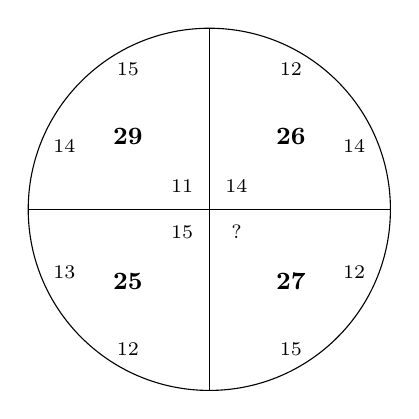
\begin{tikzpicture}[scale=1.15,font=\scriptsize]
\draw (0,0) circle(2); \draw (-2,0)--(2,0); \draw (0,-2)--(0,2);
\node at (-0.9,1.55){15}; \node at (-1.6,0.7){14}; \node[font=\small\bfseries] at (-0.9,0.8){29}; \node at (-0.3,0.25){11};
\node at (0.9,1.55){12}; \node at (1.6,0.7){14}; \node[font=\small\bfseries] at (0.9,0.8){26}; \node at (0.3,0.25){14};
\node at (-1.6,-0.7){13}; \node at (-0.9,-1.55){12}; \node[font=\small\bfseries] at (-0.9,-0.8){25}; \node at (-0.3,-0.25){15};
\node at (1.6,-0.7){12}; \node at (0.9,-1.55){15}; \node[font=\small\bfseries] at (0.9,-0.8){27}; \node at (0.3,-0.25){?};
\end{tikzpicture}}
\optsfour{13}{15}{17}{19}
\answer{A}{13}
\begin{explain}
In each quadrant the centre number is the sum of the two outer numbers, and the inner (corner) number is $40-$ centre:
\begin{center}\small
\begin{tabular}{lccc}\toprule Quadrant & Outer sum & Centre & Inner $=40-$centre\\\midrule
Top-left & $15+14$ & 29 & 11\\ Top-right & $12+14$ & 26 & 14\\ Bottom-left & $13+12$ & 25 & 15\\ Bottom-right & $12+15$ & 27 & \textbf{13}\\\bottomrule
\end{tabular}
\end{center}
\end{explain}
\end{question}

\begin{question}{42}
{If UPE = SNC, then QHD = \blank{}\par}
\optsfour{NKH}{PGE}{OFB}{MKF}
\answer{C}{OFB}
\begin{explain}
Each letter moves two steps back: U$\rightarrow$S, P$\rightarrow$N, E$\rightarrow$C. So QHD $\rightarrow$ \textbf{OFB}.
\end{explain}
\end{question}

\begin{question}{43}
{An attached file with received e-mail is dangerous for:\par}
\optsone{it may carry virus}{computer hard disk gets overloaded}{it costs money to the recepient}{there is no guarantee of reaching to recepient}
\answer{A}{it may carry virus}
\begin{explain}
Attachments from unknown senders may carry \textbf{viruses or malware} (executables, macros) that infect the computer when opened.
\end{explain}
\end{question}

\begin{question}{44}
{In the domain name .org implies:\par}
\optstwo{a website}{operations research group}{commercial website}{an organization}
\answer{D}{an organization}
\begin{explain}
The top-level domain \texttt{.org} denotes an \textbf{organisation}, typically a non-profit. (\texttt{.com} = commercial, \texttt{.edu} = education, \texttt{.gov} = government.)
\end{explain}
\end{question}

\begin{question}{45}
{URL means:\par}
\optstwo{Uniform Resource Locator}{Unique Resource Location}{Universal Recommended Location}{United Resource for Learners}
\answer{A}{Uniform Resource Locator}
\begin{explain}
\textbf{URL} is \textbf{Uniform Resource Locator}.
\end{explain}
\end{question}

\begin{question}{46}
{In a democratic institution most of the communication is:\par}
\optsfour{Vertical}{Horizontal}{Spiral}{Unidimensional}
\answer{B}{Horizontal}
\begin{explain}
In a democratic institution, communication is predominantly \textbf{horizontal}: among peers and equals, participative and consultative, rather than top-down.
\end{explain}
\end{question}

\begin{question}{47}
{Which is odd one?\par}
\optstwo{Microsoft Word}{Microsoft Excel}{Microsoft Access}{Microsoft Windows}
\answer{D}{Microsoft Windows}
\begin{explain}
Word, Excel and Access are \emph{application software} (MS Office). \textbf{Windows} is an \emph{operating system}, so it is the odd one out.
\end{explain}
\end{question}

\begin{question}{48}
{Which one is the largest memory size?\par}
\optsfour{Kilobyte}{Gigabyte}{Terabyte}{Megabyte}
\answer{C}{Terabyte}
\begin{explain}
\textbf{Terabyte} is the largest: TB $>$ GB $>$ MB $>$ KB.
\end{explain}
\end{question}

\begin{question}{49}
{In most of the Indian big cities, the dominant source of air pollution is:\par}
\optstwo{vehicular traffic}{household smoke}{thermal power plant}{suburban trains}
\answer{A}{vehicular traffic}
\begin{explain}
In big Indian cities, \textbf{vehicular traffic} is the dominant source of air pollution (NO$_x$, CO, particulate matter), especially at ground level where people breathe.
\end{explain}
\end{question}

\begin{question}{50}
{Which of the following is not biodegradable?\par}
\optsfour{Vegetables}{Human bones}{Earthworms}{Iron rust}
\answer{D}{Iron rust}
\begin{explain}
Vegetables, bones and earthworms are organic and are decomposed by microbes. \textbf{Iron rust} (hydrated iron oxide) is inorganic and not biodegradable.
\end{explain}
\end{question}

\begin{question}{51}
{Which of the following is least likely to be an effect of Global Warming?\par}
\optsone{Loss of fertile delta regions for agriculture}{Change in global patterns for precipitation}{Decreased rate of photosynthesis in vegetation}{Increased frequency of hurricanes}
\answer{C}{Decreased rate of photosynthesis in vegetation}
\begin{explain}
Global warming is expected to cause loss of deltas (sea-level rise), changed precipitation and more intense hurricanes. Higher CO$_2$ tends to \emph{increase} photosynthesis (the CO$_2$ fertilisation effect), so a \textbf{decreased rate of photosynthesis} is the least likely effect.
\end{explain}
\end{question}

\begin{question}{52}
{Which of the following is used in pencils?\par}
\optsfour{Graphite}{Silicon}{Charcoal}{Phosphorous}
\answer{A}{Graphite}
\begin{explain}
The ``lead'' of a pencil is \textbf{graphite} (a form of carbon) mixed with clay. Pencils contain no lead.
\end{explain}
\end{question}

\begin{question}{53}
{The major cause of Tsunamis in the sea is:\par}
\optsfour{Winds}{Earthquakes}{Volcanoes}{Climate change}
\answer{B}{Earthquakes}
\begin{explain}
Most tsunamis are generated by undersea \textbf{earthquakes} (sudden displacement of the sea floor), e.g.\ the 2004 Indian Ocean tsunami (magnitude 9.1).
\end{explain}
\end{question}

\begin{question}{54}
{Sardar Sarovar Project is situated on the river:\par}
\optsfour{Krishna}{Godavari}{Narmada}{Yamuna}
\answer{C}{Narmada}
\begin{explain}
The \textbf{Sardar Sarovar} dam is on the \textbf{Narmada} river at Kevadia (Ekta Nagar), Gujarat, near the Statue of Unity.
\end{explain}
\end{question}

\begin{question}{55}
{What is the basic concern of Rashtriya Uchchatar Shiksha Abhiyan?\par}
\optsone{To get over low enrolment in higher education}{To improve achievement level of students in university exams}{To improve the facilities for girls in colleges and universities}{To provide NET qualified teachers to universities and colleges}
\answer{A}{To get over low enrolment in higher education}
\begin{explain}
\textbf{RUSA} (2013) aims at improving access, equity and quality in state higher education. Its basic concern is to raise \textbf{GER, i.e.\ to overcome low enrolment} in higher education (target 32\% by the end of the 12th Plan).
\end{explain}
\end{question}

\begin{question}{56}
{Rashtriya Uchchatar Shiksha Abhiyan (RUSA) is to fund the states for higher education. What is the ratio of funds between Central and State governments?\par}
\optstwo{75\% Centre : 25\% State Governments}{65\% Centre : 35\% State Governments}{100\% Centre}{78\% Centre : 22\% State Governments}
\answer{A}{75\% Centre : 25\% State Governments}
\keynote{Under the approved RUSA scheme the Centre--State ratio was 65:35 for general-category states (90:10 for special-category states). The official key nevertheless gives (A).}
\begin{explain}
The official key gives \textbf{75\% Centre : 25\% State}, the funding pattern cited in early RUSA documents. RUSA funds reach state universities and colleges through state higher-education councils.
\end{explain}
\end{question}

\begin{question}{57}
{What does PPP stand for in higher education policy perspective?\par}
\optstwo{Policy Perspective Plan}{People's Planning for Participation}{Public Private Partnership}{Privatisation Policy Pattern}
\answer{C}{Public Private Partnership}
\begin{explain}
In higher-education policy, \textbf{PPP} means \textbf{Public--Private Partnership}: collaboration between government and private players to expand and improve institutions.
\end{explain}
\end{question}

\begin{question}{58}
{What has been the purpose of introducing NET as basic qualification for recruitment of teachers in higher education?\par}
\optsone{Ensure that curriculum is centralized in all the Indian Universities}{Ensuring that teaching takes place in the classes in higher education}{Ensure that teachers' knowledge improves}{Ensure merit in recruitment of teachers in higher education}
\answer{D}{Ensure merit in recruitment of teachers in higher education}
\begin{explain}
UGC introduced the \textbf{NET} (1989) as the minimum eligibility for Assistant Professors to \textbf{ensure merit and uniform standards in the recruitment of teachers}.
\end{explain}
\end{question}

\begin{question}{59}
{Why does Gross Enrolment Ratio (GER) sometimes go beyond 100 in higher education?\par}
\optsone{Due to number of repeaters and number of younger and older age group students}{Due to larger enrolment in distance education courses}{Due to continuous increase in population of particular age group students}{Due to government policies of access in higher education}
\answer{A}{Due to number of repeaters and number of younger and older age group students}
\begin{explain}
GER $=$ enrolment of \emph{all ages} in a level $\div$ population of the official age group. Because \textbf{repeaters and under- or over-age students} are counted in the numerator, GER can exceed 100.
\end{explain}
\end{question}

\begin{question}{60}
{Which of the following is a challenge for governance in higher education?\par}
\optsone{Getting NET qualified teachers}{Getting students for different courses}{Preparing syllabi for different courses}{Meeting funding requirements}
\answer{D}{Meeting funding requirements}
\begin{explain}
Governance of higher education faces the challenge of \textbf{meeting funding requirements}: institutional finance, autonomy linked to funding, and efficient use of resources.
\end{explain}
\end{question}
